


\title{Version control}
\subtitle{How GIT can make your life better}
\author{Simon R.~White}
\institute{MRC Biostatistics Unit, University of Cambridge}
\date{2018/Apr/11}

\begin{document}

\maketitle








\begin{frame}{Outline and aims}
  
  \begin{block}{Outline}
    \begin{itemize}
    \item Version control
    \item GIT fundamentals (the why)
    \item GIT basics (the how)
    \item Advanced GIT
    \end{itemize}
  \end{block}

  \begin{block}{Aims}
    Open to discussion and happy to change focus
    \begin{itemize}
    \item Understand concepts of version control
    \item Highlight reasons to spend the time/effort to embrace
      version control
    \end{itemize}
  \end{block}

\end{frame}



\begin{frame}{Backing up and version control}

  Version control and backing up your work are different:
  
  \begin{itemize}

  \item A backup is needed if, say, you lose your laptop\\within the
    BSU our home directories are backup up
  \item Version control is about managing and recording changes to a specific set of files/documents
  \end{itemize}

  \pause

  What you might be doing at the moment:

  \begin{itemize}
  \item {\usebeamercolor[fg]{item}Dropbox:}\\a backup - does include some version
    control (ish)
  \item {\usebeamercolor[fg]{item}Saving copies:}\\`\texttt{Paper Apr10.tex}', `\texttt{Paper Apr8 +
      SWcomment.tex}', etc.
  \end{itemize}

  \pause

  \alert{Question: what if your laptop died right now?}

\end{frame}


\begin{frame}{When to use version control?}
  
  \begin{itemize}
  \item Most version control systems, including GIT, excel with
    text-based files
  \item Microsoft Word (and Excel) are not great formats for this
    \begin{itemize}
    \item MS Word has its own track-changes features
    \end{itemize}
  \end{itemize}


\end{frame}


\begin{frame}{A proper version control system}
  
  \begin{block}{Benefits}
    \begin{itemize}
    \item Robust record of work/code
    \item Collaborative work can be a lot easier
    \end{itemize}
  \end{block}

  \begin{block}{Issues}
    \begin{itemize}
    \item Need to learn to use new software
    \item Can complicate things as you shift the way you work
    \end{itemize}
  \end{block}

\end{frame}


\begin{frame}{Options}
  
  \begin{itemize}
  \item subversion
  \item Mercurial
  \item GIT
  \item Many others
  \end{itemize}

  Features to consider:
  \begin{itemize}
  \item Server-Client or Distributed
  \item Direction of the wind today
  \end{itemize}

\end{frame}


\begin{frame}{Ways to use GIT}
  
  \begin{itemize}
  \item command line
  \item graphical user interface (GUI)\\\url{https://git-scm.com/download/gui/windows}
  \end{itemize}

  Today we'll do a little of both.


\end{frame}


\begin{frame}{GIT fundamentals}
  
  \begin{itemize}
  \item Every repository contains the complete history\\(this means
    they can get big)
  \item There are three parts to work with
    \begin{adjustbox}{center}
      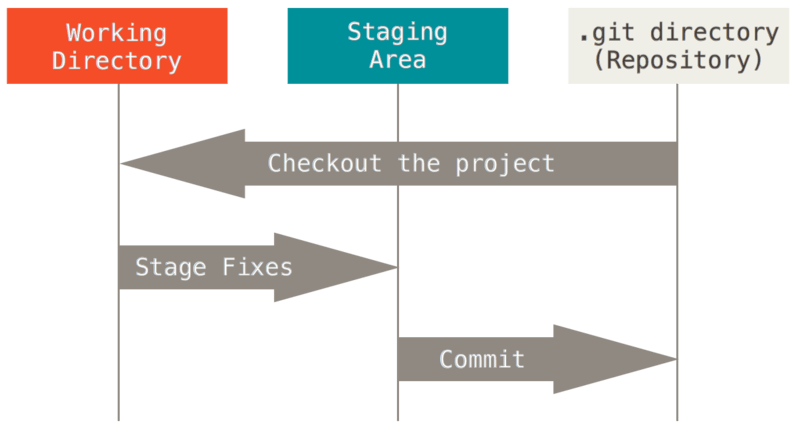
\includegraphics[width=0.6\textwidth]{img/areas}
    \end{adjustbox}
  \item A repository on its own is not safe
  \end{itemize}


\end{frame}


\begin{frame}{Online resources}
  
  \begin{itemize}
  \item \url{https://git-scm.com/book/en/v2/Getting-Started-About-Version-Control}


  \item \url{https://git-scm.com/book/en/v2/Git-Basics-Getting-a-Git-Repository}
  \end{itemize}


  

\end{frame}


\begin{frame}[fragile]{GIT basic commands}

  \begin{itemize}
  \item make a new repository
\begin{verbatim}
git init
\end{verbatim}
  \item staging files
\begin{verbatim}
git add
git add -u ./
git add -A ./
\end{verbatim}
  \item commit change-set to repo
\begin{verbatim}
git commit -m"testing"
\end{verbatim}
  \end{itemize}
\end{frame}


\begin{frame}[fragile]{GIT overviews}

  \begin{itemize}
  \item Details of commits
\begin{verbatim}
git log
git log -n2
git log --name-status -n2
\end{verbatim}
  \item Details of current working directory
\begin{verbatim}
git status
\end{verbatim}
  \item History
\begin{verbatim}
git hist
\end{verbatim}
{\fontsize{6}{8}{\begin{verbatim}
## Config file
[alias]
    hist   = log --all --pretty=format:\"%C(auto)%h%Creset %C(magenta)%ad%Creset 
                                         |%C(auto)%d%Creset %C(auto)%s%Creset 
                                         %C(blue)[%an]%Creset %C(green)<%cr>%Creset\" 
                 --graph --date=short
\end{verbatim}}}
  \end{itemize}
\end{frame}




\begin{frame}[fragile]{GIT basic commands}

  \begin{itemize}
  \item make a new repository
\begin{verbatim}
git init
\end{verbatim}
  \item staging files
\begin{verbatim}
git add
git add -u ./
git add -A ./
\end{verbatim}
  \item commit change-set to repo
\begin{verbatim}
git commit -m"testing"
\end{verbatim}
  \end{itemize}
\end{frame}



\begin{frame}
  \begin{beamercolorbox}[sep=1em]{frametitleback}
    \centering
    \begin{Huge}
      {\usebeamercolor[fg]{frametitle}Reasons to use GIT}
    \end{Huge}
  \end{beamercolorbox}

\end{frame}


\begin{frame}[fragile]{Easily integrate with latexdiff}

Config file:
\begin{verbatim}
[alias]
    wdiff = diff --color-words --ignore-all-space
    ldiff = difftool -y -t latex
[difftool.latex]
    cmd = latexdiff "$LOCAL" "$REMOTE"
\end{verbatim}
  
\begin{verbatim}
git diff v1.0..v1.1 Outline.tex
git ldiff v1.0..v1.1 Outline.tex > LDIFF.tex
\end{verbatim}

\end{frame}


\begin{frame}[fragile]{GNU Meld for viewing differences}

Config file:
\begin{verbatim}
[alias]
    mdiff = difftool -t meld
\end{verbatim}
  
\begin{verbatim}
git mdiff v1.0..v1.1 Outline.tex
\end{verbatim}

\end{frame}



\begin{frame}[fragile]{Ignoring files (for cleaner repositories)}
  
  See GIT-talk repo

  \itshape\color{gray}
  The status command can get quite busy (especially with unnecessary
  \LaTeX files).
\begin{verbatim}
## create a file in repository called .gitignore
## list patterns to ignore, such as

*.out
*.aux


## run the status command to see difference
git status
\end{verbatim}


\end{frame}



\begin{frame}[fragile]{Working with multiple clones}
  
  See GIT-talk repo (and clones)

  \vspace{1em}

  \itshape\color{gray}
  Using this example repository, make a clone
\begin{verbatim}
git clone /path/to/repo/on/your/computer NEW-NAME
\end{verbatim}


\begin{verbatim}
## within clone

git remote -v ## shows remotes this repo is aware of

git fetch origin ## fetch commits from remote repo
\end{verbatim}


\begin{verbatim}
## within first repo

git remote add DAVE /path/to/NEW-NAME

git fetch DAVE
\end{verbatim}



\end{frame}



\begin{frame}[fragile]{Merges with multiple committers}
  
  See NSPN-live repo

  \itshape\color{gray}
  Using this example repository
\begin{verbatim}
## bring branches together
git checkout master

git diff git-magic^..git-magic
## or
git diff 8c0c706..04aebee

git branch TEST
git checkout TEST

git merge git-magic
\end{verbatim}


\end{frame}

\begin{frame}[fragile]{Cloned repos for code}
  
  See FM-p repos


  \itshape\color{gray}
  Create local clones of repository for running code, while continuing
  to edit the original
\begin{verbatim}
git clone /path/to/repo Cluster-cpy-A
\end{verbatim}


\end{frame}


\begin{frame}[fragile]{Dropbox trick (advanced paths)}
  
  See NSPN dropbox+repos


  \itshape\color{gray}
  By default the {\upshape\texttt{.git}} folder sits inside the working
  directory, but it can be elsewhere. For Dropbox, we can host a repo
  inside a dropbox folder without the associated {\upshape\texttt{.git}}
\begin{verbatim}
git --git-dir=/path/to/.git 
    --work-tree=/path/to/working-directory
\end{verbatim}


\end{frame}





% \begin{frame}{EXAMPLE IMAGE SLIDE}
%   \begin{adjustbox}{center}
%     \includegraphics[width=0.8\textwidth]{FILENAME}
%   \end{adjustbox}
%   \begin{adjustbox}{center}
%     \footnotesize{\usebeamercolor[fg]{item}Fig:} \emph{CAPTION}
%   \end{adjustbox}
% \end{frame}









\end{document}

%%% Local Variables: 
%%% mode: latex
%%% TeX-master: "SWhite-slides"
%%% End: 
